%%%%%%%%%%%%%%%%%%%%%%%%%%%%%%%%%%%%%%%%%%%%%%%%%%%%%%%%%%%%%%%%%%%%%%%%%%%%%%%%%%%%%%%%%%%%%%%%%%%%%%%%%%%%%%%%%%%%%%%%%%%%%%%%%%%%%%%%%%%%%%%%%%%%%%%%%%%
% This is just an example/guide for you to refer to when producing your supplementary material for your Frontiers article.                                 %
%%%%%%%%%%%%%%%%%%%%%%%%%%%%%%%%%%%%%%%%%%%%%%%%%%%%%%%%%%%%%%%%%%%%%%%%%%%%%%%%%%%%%%%%%%%%%%%%%%%%%%%%%%%%%%%%%%%%%%%%%%%%%%%%%%%%%%%%%%%%%%%%%%%%%%%%%%%

%%% Version 2.5 Generated 2018/06/15 %%%
%%% You will need to have the following packages installed: datetime, fmtcount, etoolbox, fcprefix, which are normally inlcuded in WinEdt. %%%
%%% In http://www.ctan.org/ you can find the packages and how to install them, if necessary. %%%
%%%  NB logo1.jpg is required in the path in order to correctly compile front page header %%%

\documentclass[utf8]{frontiers_suppmat} % for all articles
\usepackage{url,hyperref,lineno,microtype,subcaption}
\usepackage[onehalfspacing]{setspace}
\graphicspath{{figures/}}
\usepackage{xr}

\makeatletter
\newcommand*{\addFileDependency}[1]{% argument=file name and extension
  \typeout{(#1)}
  \@addtofilelist{#1}
  \IfFileExists{#1}{}{\typeout{No file #1.}}
}
\makeatother

\newcommand*{\crossreference}[1]{%
    \externaldocument{#1}%
    \addFileDependency{#1.tex}%
    \addFileDependency{#1.aux}%
}
\crossreference{frontiers}


\begin{document}
\onecolumn
\firstpage{1}

\title[Supplementary Material]{{\helveticaitalic{Supplementary Material}}}
\maketitle
% \section{Supplementary Data}
% Supplementary Material should be uploaded separately on submission. Please include any supplementary data, figures and/or tables. All supplementary files are deposited to FigShare for permanent storage and receive a DOI.

% Supplementary material is not typeset so please ensure that all information is clearly presented, the appropriate caption is included in the file and not in the manuscript, and that the style conforms to the rest of the article. To avoid discrepancies between the published article and the supplementary material, please do not add the title, author list, affiliations or correspondence in the supplementary files.

\appendix
\section{Network architecture}
\label{sec:supp:architecture}
The network is a fully convolutional residual network \cite[]{He2016DeepRecognition} composed recursively as described in Section \ref{sec:methods:formulation} to integrate in time.
The final architecture used in the heterogeneous case and shown in Figure \ref{fig:2}, is as follows:
The input to the neural network is a $2 \times 4 \times 256 \times 256$ tensor, representing two temporal instants, 5ms apart, of the three state variables and the diffusivity map, $\sigma$, which is constant throughout time. We solve the problem in a rectangular domain discretised to a uniform $256 \times 256$ grid.
Except for the last operation, all convolutions are performed on the last three dimensions of the tensor.
The first layer is a linear projection of the four input channels $\langle v, w, u, \sigma \rangle$ to a higher dimensional space, obtained by convolving the input with 16 kernels of size $(4, 3, 3)$ with stride $(1, 1, 1)$ to obtain a tensor of shape $16 \times 4 \times 256 \times 256$.
It follows a serial sequence of 20 three-dimensional convolutional layers with 16 kernels of size $(4, 3, 3)$, stride $(1, 1, 1)$ and padding $(0, 2, 2)$, interleaved with non linearities and residual connections.
To mitigate the dying ReLU problem, and guarantee full support in $\mathbb{R}$ to each convolutional block, we replaced the ReLUs non-linearities of the standard ResNet \cite[]{He2016DeepRecognition} with exponential linear units (ELUs) \cite[]{Clevert2016FastELUs}.
The model ends with two additional linear projections. The former compresses the 16 features into a single one, resulting into a tensor of shape $1 \times 4 \times 256 \times 256$.
The latter transforms the tensor into its final shape $1 \times 3 \times 256 \times 256$ to match the three state variables.


\section{Optimisation details}
\label{sec:supp:optimisation}
We use the adaptive momentum method \cite[]{Kingma2015Adam:Optimization} to perform parameter updates, with $\beta_1=0.9$, $\beta_2=0.999$ and $\epsilon=10^{-8}$, and a mini-batch size of 16 samples.
To mitigate the exploding gradient problem \cite[]{Bengio1994LearningDifficult} we use gradient clipping \cite[]{Pascanu2013OnNetworks} with norm 1.
To control the gradient bias due to bootstrapping in time we use full backpropagation through time (BTT) \cite[]{P.J.Werbos1990BackpropagationIt}, instead of its more usual truncated form (TBTT) \cite[p. 14]{jaeger2002tutorial}, and circumvent memory problems using function checkpointing.
This method effectively trades memory for floating point operations per second by recomputing some of the linearisation points during reverse mode differentiation.
The optimisation does not use any teacher forcing \cite[]{Williams1989ANetworks} strategy.
The training of experimental models, and an empirical estimation of the effective range of the hyperparameters, is performed on a cluster of 8 Nvidia Quadro RTX6000, with a batch size of 128.
These preliminary experimental models are evaluated at a cutoff time of 24 hours.
The final model, which we use throughout the experiments, is trained for 120 hours on two Nvidia GeForce GTX 1080 Ti with a batch size of 16 samples.
To balance computation times and gradient bias, the network is optimised using 5-step rollouts, 5ms each, corresponding to a total of 25ms.

Adding the spatial gradient loss \cite[]{kim2019deep,Lino2020SimulatingNetworks} helped to greatly reduce these artifacts after only 2 hours in the optimisation process.
initialisation
Canonical initialisation methods for residual networks \cite[]{Zhang2019FixupNormalization}, did not help improve the convergence rate. The lack of improvement might be attributed to the relative shallowness of the proposed network, being composed of only 20 residual layers.
% fixed point bias
The bootstrapping of action potential dynamics, that is, the prediction of future states from predicted past states, introduces a bias in the gradient estimation, causing the loss function to spike and SGD to diverge.
To remove the bias, we found it effective to replace the commonly used practice of truncated backpropagation through time \cite[]{jaeger2002tutorial} with full backpropagation through time \cite[]{P.J.Werbos1990BackpropagationIt}. The higher memory requirements of BTT have been circumvented using function checkpointing.
% variance
Choosing BTT over TBTT effectively traded gradient bias for higher variance.
This symptom is particularly clear when the loss is below $0.2$, that is, when approaching the fixed point.
Reducing the learning to $10^{-4}$ marginally helped reduce the variance at the cost of a lower convergence rate, albeit overall insufficient.
Instead, we observed that clipping the gradient to norm $1$ greatly contributed to reducing spiking in the loss function.


\section{Data preprocessing}
\label{sec:supp:preprocessing}
To avoid exceeding the GPU memory limits we rescale the input sequences from $1200 \times 1200$ to $256 \times 256$.
The three variables in the Fenton-Karma model are already normalised in the $[0, 1]$ range. 
Considering the different order of magnitude of the tissue diffusivity, to encourage the network to pay attention to the diffusivity map, we rescale only that to the same order of magnitude as the other state variables. The resulting diffusivity is in the range [0.05, 0.5].


\section{Pilot studies on homogeneous diffusivity}
\label{sec:supp:homogeneous}
To evaluate the choice of the architecture, we performed some pilot studies on the efficacy of the ResNet to approximate the monodomain equation in conditions of homogeneous conductivity. We refer to this model as the \textit{h-FK} model.


\subsection{Dataset generation}
\label{sec:supp:homogeneous:data}
The \textit{h-FK} model is trained on a separate dataset, named \textit{h-FKset}, which is different from the one used in the rest of the paper. 
This dataset is generated using the Fenton-Karma monodomain model with homogeneous diffusivity. It contains 3 sequences, each 2000ms long, sampled at 5ms intervals. 
All sequences are generated using parameter set 3 from \cite{Fenton2002}, but each follows a different stimulation protocol. 
The first protocol (\textit{spiral}) is a cross-field protocol consisting of two linear waves incoming from orthogonal directions, 350ms apart.
The second protocol (\textit{three points}) consists of three rectangular stimuli, 350ms apart, in three different positions. The stimuli are designed such that one occurs just after the underling tissue has repolarised to allow the formation of spiral waves. 
The third protocol (\textit{heartbeat}) consists of a periodic linear wave incoming from a fixed direction, with a period of 400ms. 
We choose this experimental setup to generate a dataset with a wide dynamical range without relying on variable diffusivity maps.

\subsection{Spectral analysis}
\label{sec:supp:homogeneous:spectral}
When evaluating neural network models trained on the \textit{h-FKset} dataset, we use a Fourier transform-based measure to compare the neural network predictions and the \textit{CardiAX} simulations. Given a spatio-temporal sequence, we compute the magnitude of the discrete 3D Fourier transform of each spatio-temporal sequence, either as predicted by the neural network or simulated by \textit{CardiAX}. The magnitude is normalised to have unit sum. Then we project the spectral magnitude onto a set of delta-like functions ($g_k(f_x,f_y,f_t$) where $f_x,f_y,f_t$ are the spatial and temporal frequencies), each represented as the probability distribution function of a Gamma distribution. By varying the shape parameter ($k$) of each Gamma distribution, we are able to weigh contributions from different frequency bands. Specifically we use $18$ different values of $k$, equally spaced between $10$ and $180$ (included). We use a scale of $0.0025$ for all Gamma distributions. By construction, the functions $g_k(\cdot)$ have unit sum and are such that $g_k(f_x,f_y,f_t) = g_k(f_x^2+f_y^2)\times g_k(\|f_t\|)$. Projecting the spatio-temporal Fourier space of a short space-time sequence onto this set of Gamma distributions produces a set of scalars $\lambda_k = \sum_{f_x,f_y,f_t}{\rho(f_x,f_y,f_t)\times g_k(f_x,f_y,f_t)}$, where $\rho(f_x,f_y,f_z)$ represents the spectral magnitude at a given set of frequency coordinates $(f_x, f_y, f_z)$. We then calculate the spectral moment of order $p$ as $\sum_k{x_k^p \lambda_k}$, where $x$ is the peak of a one-dimensional Gamma distribution with shape parameter $k$. We use three spectral moments (with $p=1,2,3$) as a ``spectral signature'' of a given spatio-temporal sequence.

We then leverage this signature to identify those sequences generated either by \textit{CardiAX} or by the neural network trained on the homogeneous conductive medium that are most distinctive of their own category. That is, we look for those \textit{CardiAX} simulations that are closer to other simulations than to any neural network prediction, and vice-versa. To do this, we concatenate the spectral signatures of both \textit{CardiAX} simulations and neural network predictions. For each sequence we then find the $25$ nearest neighbours and count how many of them belong to the same category as the sequence under analysis. We define a sequence as being ``isolated'' if all its neighbours belong to the same category as the sequence itself.

\subsection{Results}
% "old" model figures
\begin{figure}[!htp]
\centering
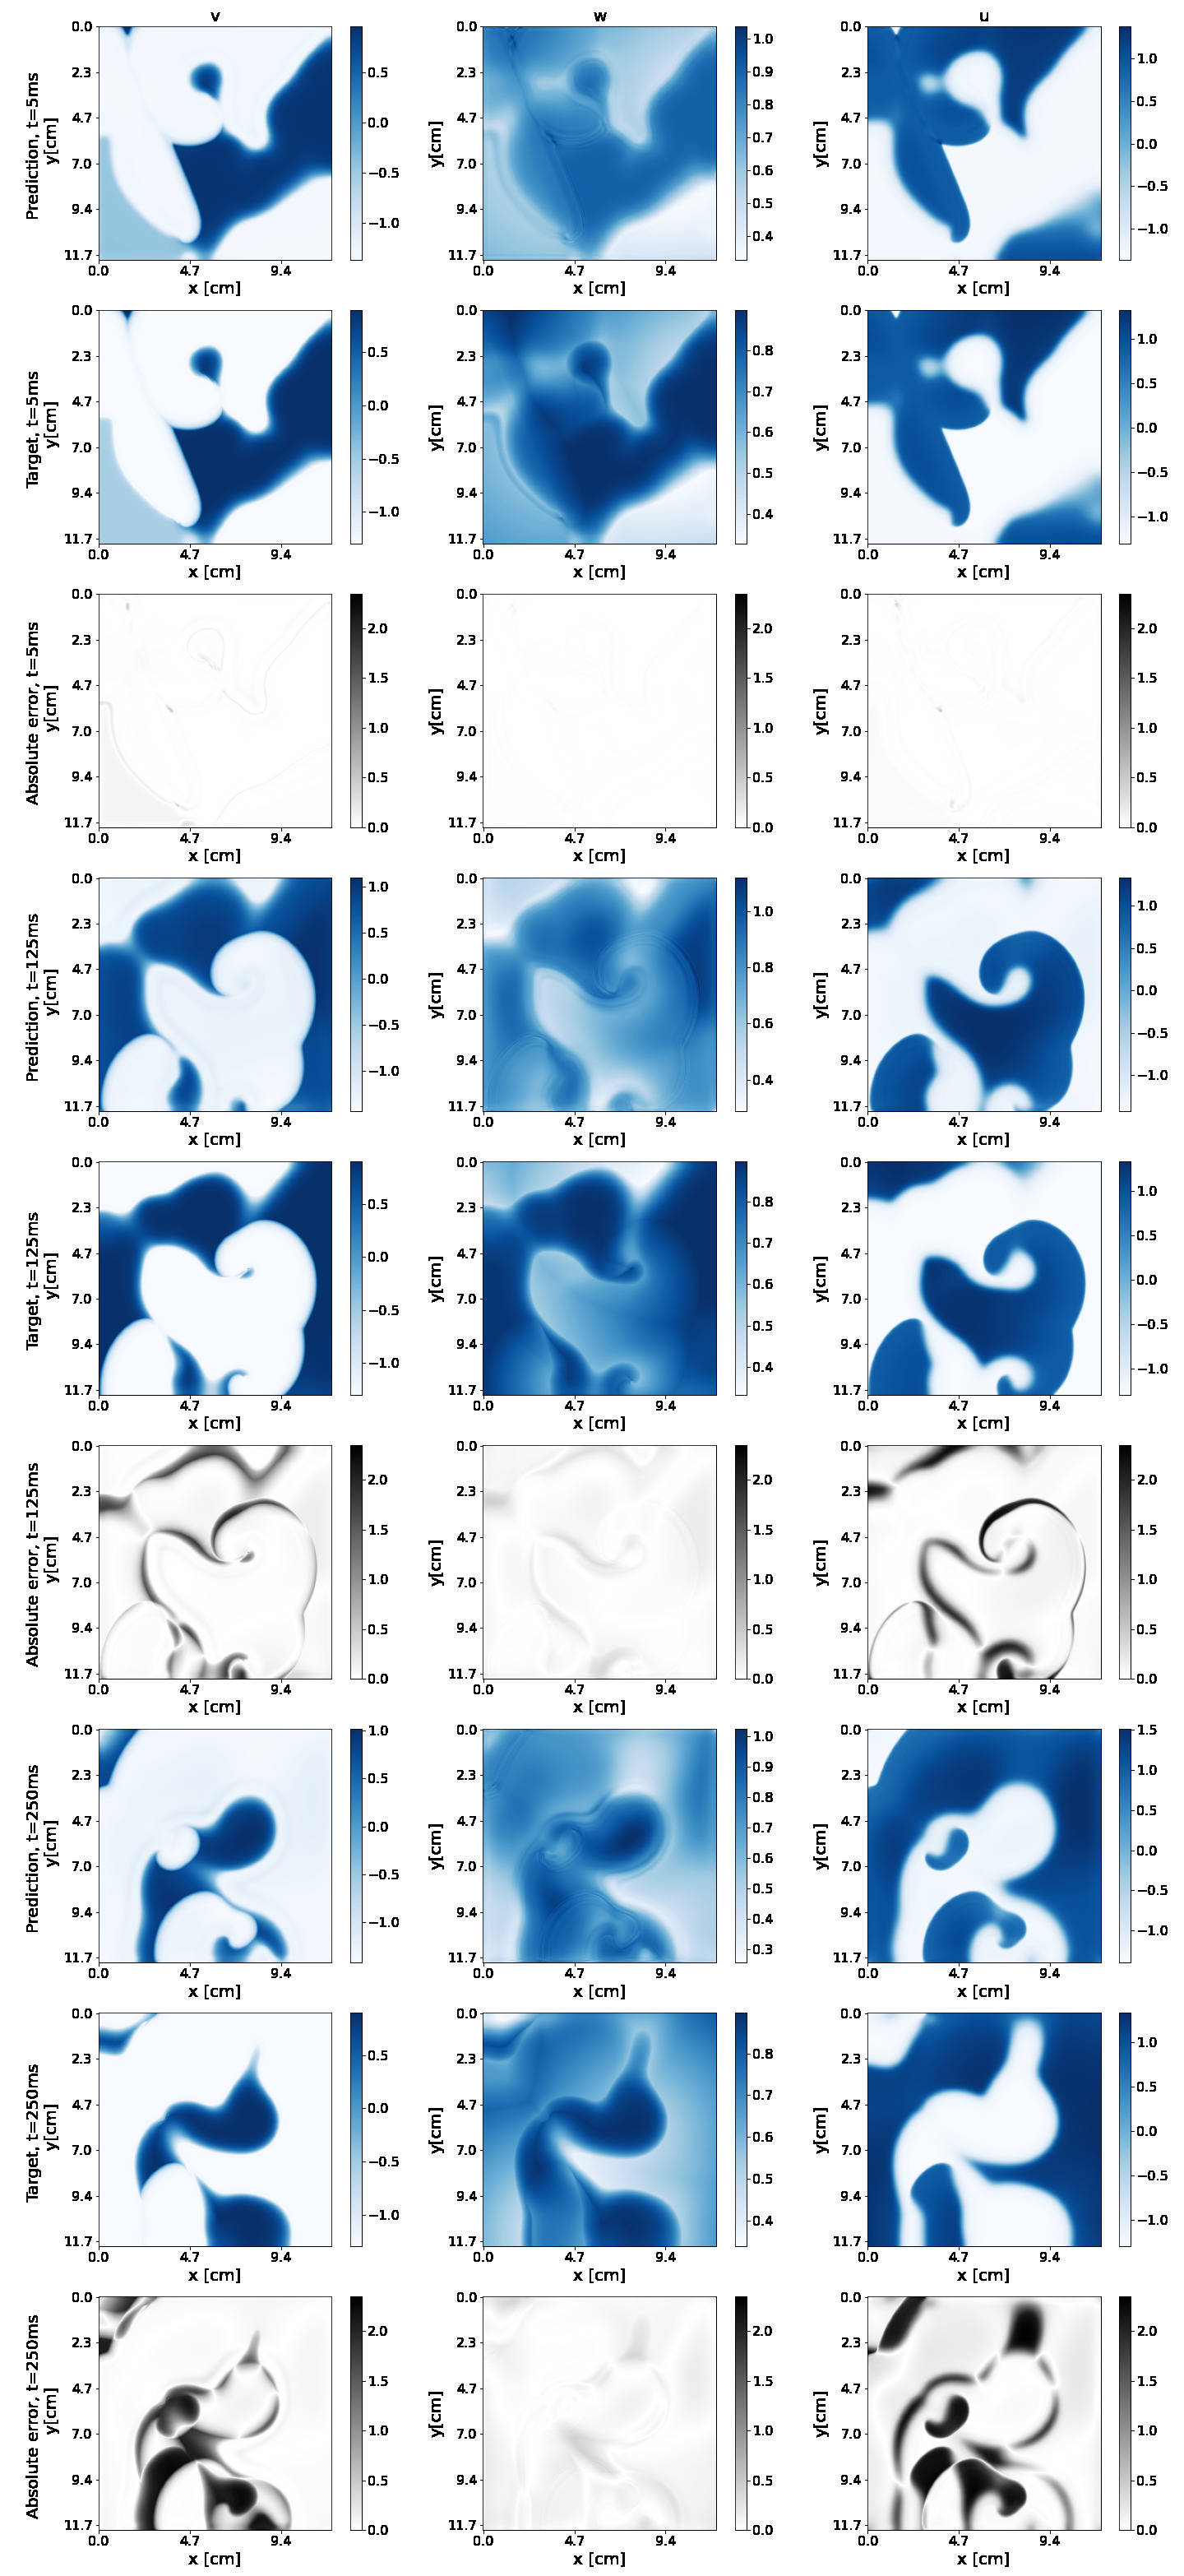
\includegraphics[width=.52\textwidth]{figures/old_figures/Figure-3.jpg}
 \caption{Results of the qualitative analysis of the pilot studies on homogeneous diffusivity with small approximation errors. The neural network, trained only on the \textit{h-FKset} dataset, is used to predict the state of the system up to $250$ms ahead, that is $50$ time steps, $5$ms apart. We show here the predictions at three different time steps ($t=5ms$, $t=130ms$ and $t=250ms$). Images depict sequence predictions, where each triplet of rows presents a different time horizon. The first row of each triplet shows the neural network model inference, the second the \textit{CardiAX} solution, and the third the $L_1$ error between the two.
 These predictions represent small approximation errors between the standard and the neural network solvers.}\label{fig:scarfreequalitativemin}
\end{figure}

\begin{figure}[!htp]
\centering
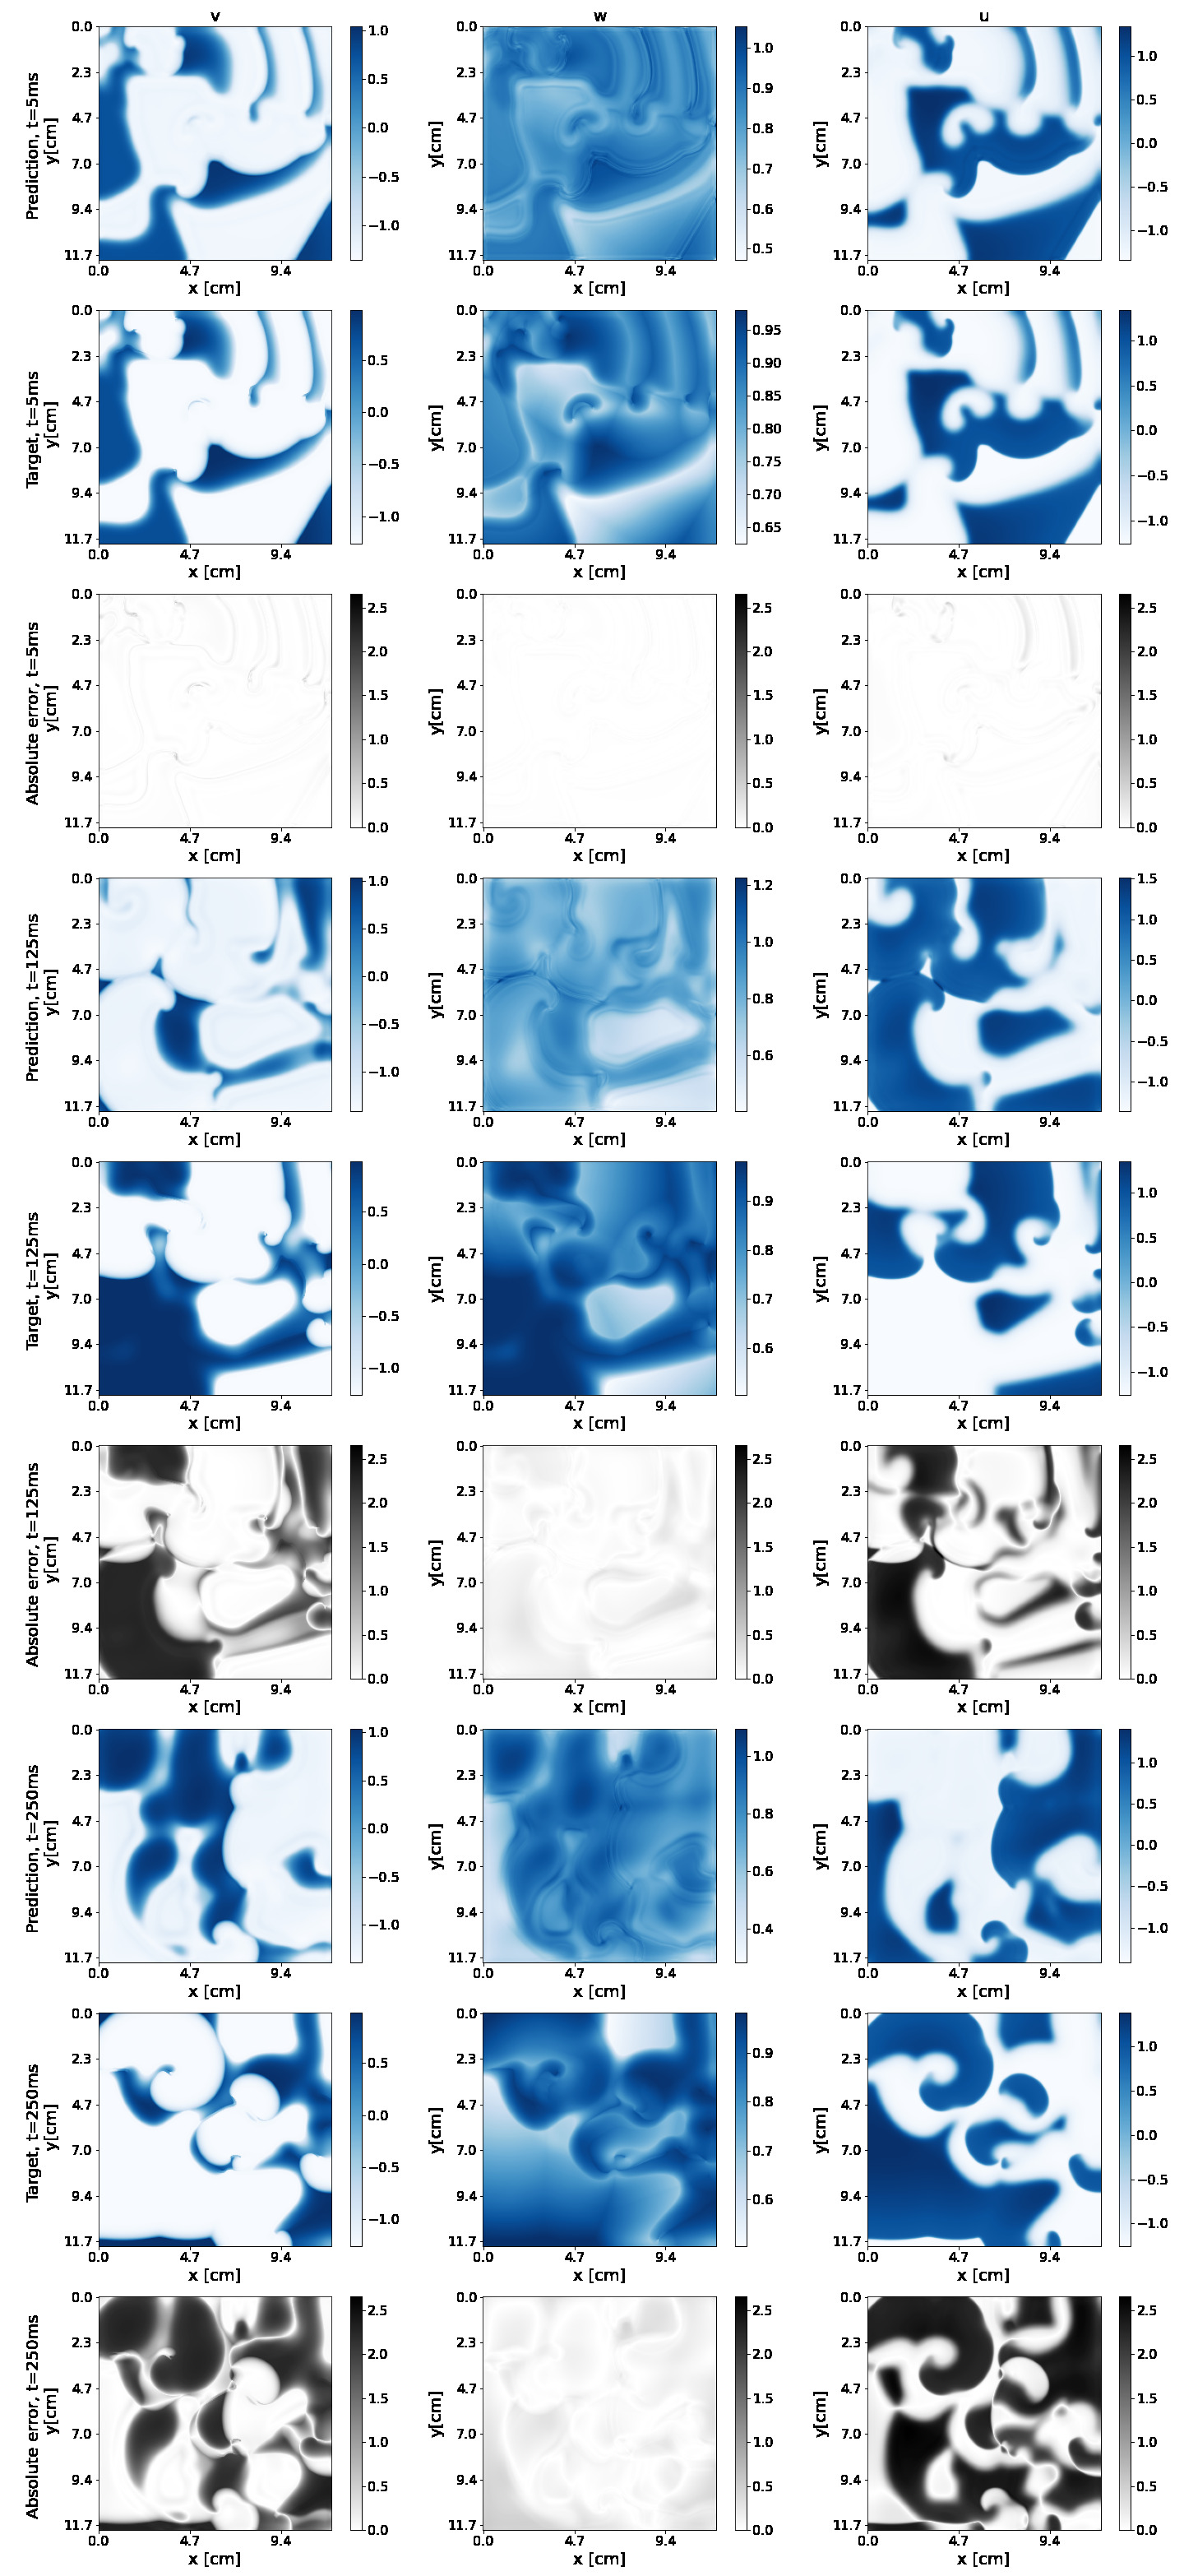
\includegraphics[width=.52\textwidth]{figures/old_figures/Figure-4.jpg}
\caption{Results of the qualitative analysis of the pilot studies on homogeneous diffusivity with large approximation errors. The neural network, trained only on the \textit{h-FKset} dataset, is used to predict the state of the system up to $250$ms ahead, that is $50$ time steps, $5$ms apart. We show here the predictions at three different time steps ($t=5ms$, $t=130ms$ and $t=250ms$). Images depict sequence predictions, where each triplet of rows presents a different time horizon. The first row of each triplet shows the neural network model inference, the second the \textit{CardiAX} solution, and the third the $L_1$ error between the two.
These predictions represent large approximation errors between the standard and the neural network solvers.}\label{fig:scarfreequalitativemax}
\end{figure}

Figures~\ref{fig:scarfreequalitativemin} and~\ref{fig:scarfreequalitativemax} shows the simulated and predicted data at 3 different time horizons for two sequences, chosen as exemplars of low (Figure~\ref{fig:scarfreequalitativemin}) and large (Figure~\ref{fig:scarfreequalitativemax}) approximation errors. Both sets of predictions appear qualitatively plausible for the case of homogeneous (scar-free) propagation. However, there are some discrepancies between the time sequences generated using the standard and the neural network solvers.
In Figure~\ref{fig:scarfreequalitativemin} the error seems to concentrate around the wavefront, especially at earlier and intermediate time steps (third and sixth rows). Furthermore, both figures show how small deviations in the predictions can be amplified at later time steps, so that simulations and predictions diverge. Indeed, the error between predictions and \textit{CardiAX} simulations seems to increase with time in both sequences, as can be noted by comparing the last row of each figure with the third one.


\begin{figure}[!htp]
\centering
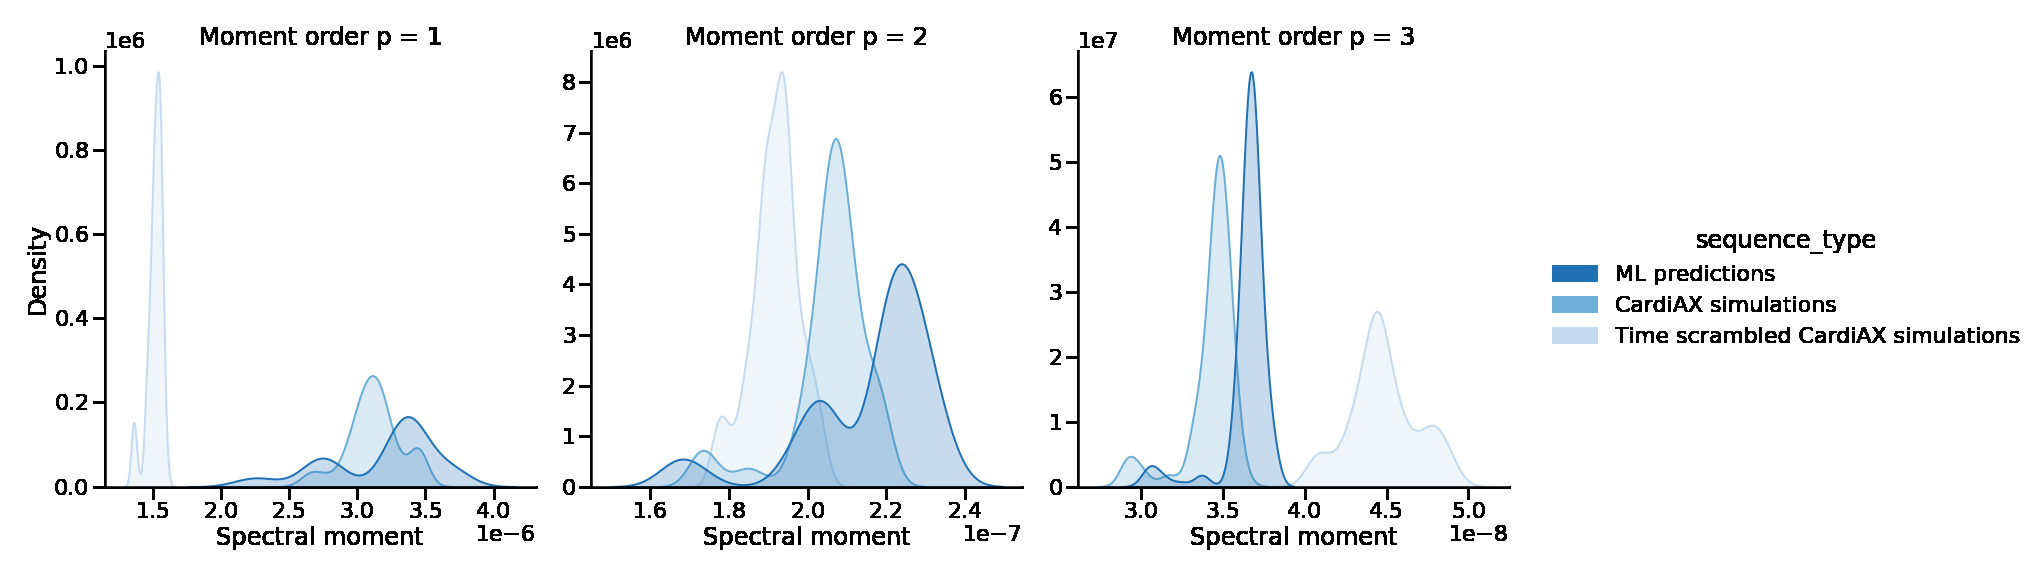
\includegraphics[width=\textwidth]{figures/old_figures/Figure-5.jpg}
\caption{
    Results of the spectral analysis of the pilot studies on homogeneous diffusivity. Each graph shows the distribution of spectral moments across different types of time sequences: neural network predictions, \textit{CardiAX} simulations and time scrambled \textit{CardiAX} simulations. Each graph shows spectral moments of a different order: $1$ (left), $2$ (centre) and $3$ (right). Note that only sequences that do not contain the onset of an external stimulus are included in the analysis. Notice how the spectral distributions of predictions and simulations have a larger overlap with each other than with the spectral distribution of the time scrambled sequences.
}\label{fig:momentssimhist}
\end{figure}

\subsubsection{Analysis using spectral moments}\label{ch:fft}
While the predictions may appear qualitatively plausible, it is possible for the sequences generated by the neural network to diverge into a different dynamical regime. In the following, we investigate the use of a Fourier transform-based metric, described in section \ref{ch:spectral}, to help quantify this qualitative difference.

We apply this measure to three different types of time sequences: the simulations generated by \textit{CardiAX}, the neural network (ML) predictions and time scrambled \textit{CardiAX} simulations. The latter are generated by randomly permuting a given simulation along its temporal axis and used as a control sequence.
%results on pilot studies
Figure~\ref{fig:momentssimhist} shows the distributions of moments across all $321$ test sequences from each condition. Each graph shows the distribution of spectral moments of a different order $p$: $p=1$ (left), $p=2$ (centre) and $p=3$ (right). Notice how the spectral distributions of the ML predictions and the original \textit{CardiAX} simulations are closer to each other than to the distribution of the time scrambled sequences. However, there are also visible differences between the distributions of spectral moments for ML predictions and \textit{CardiAX} simulations, which would suggest the existence of discrepancies between the dynamics generate by standard and the neural network solvers (similarly to what observed in Figures~\ref{fig:scarfreequalitativemin} and~\ref{fig:scarfreequalitativemax}). This result highlights how the spectral moments crucially depend on the temporal dynamics of the time series under analysis and helps justify their use to quantify differences between sequences.

\begin{figure}[tp]
\centering
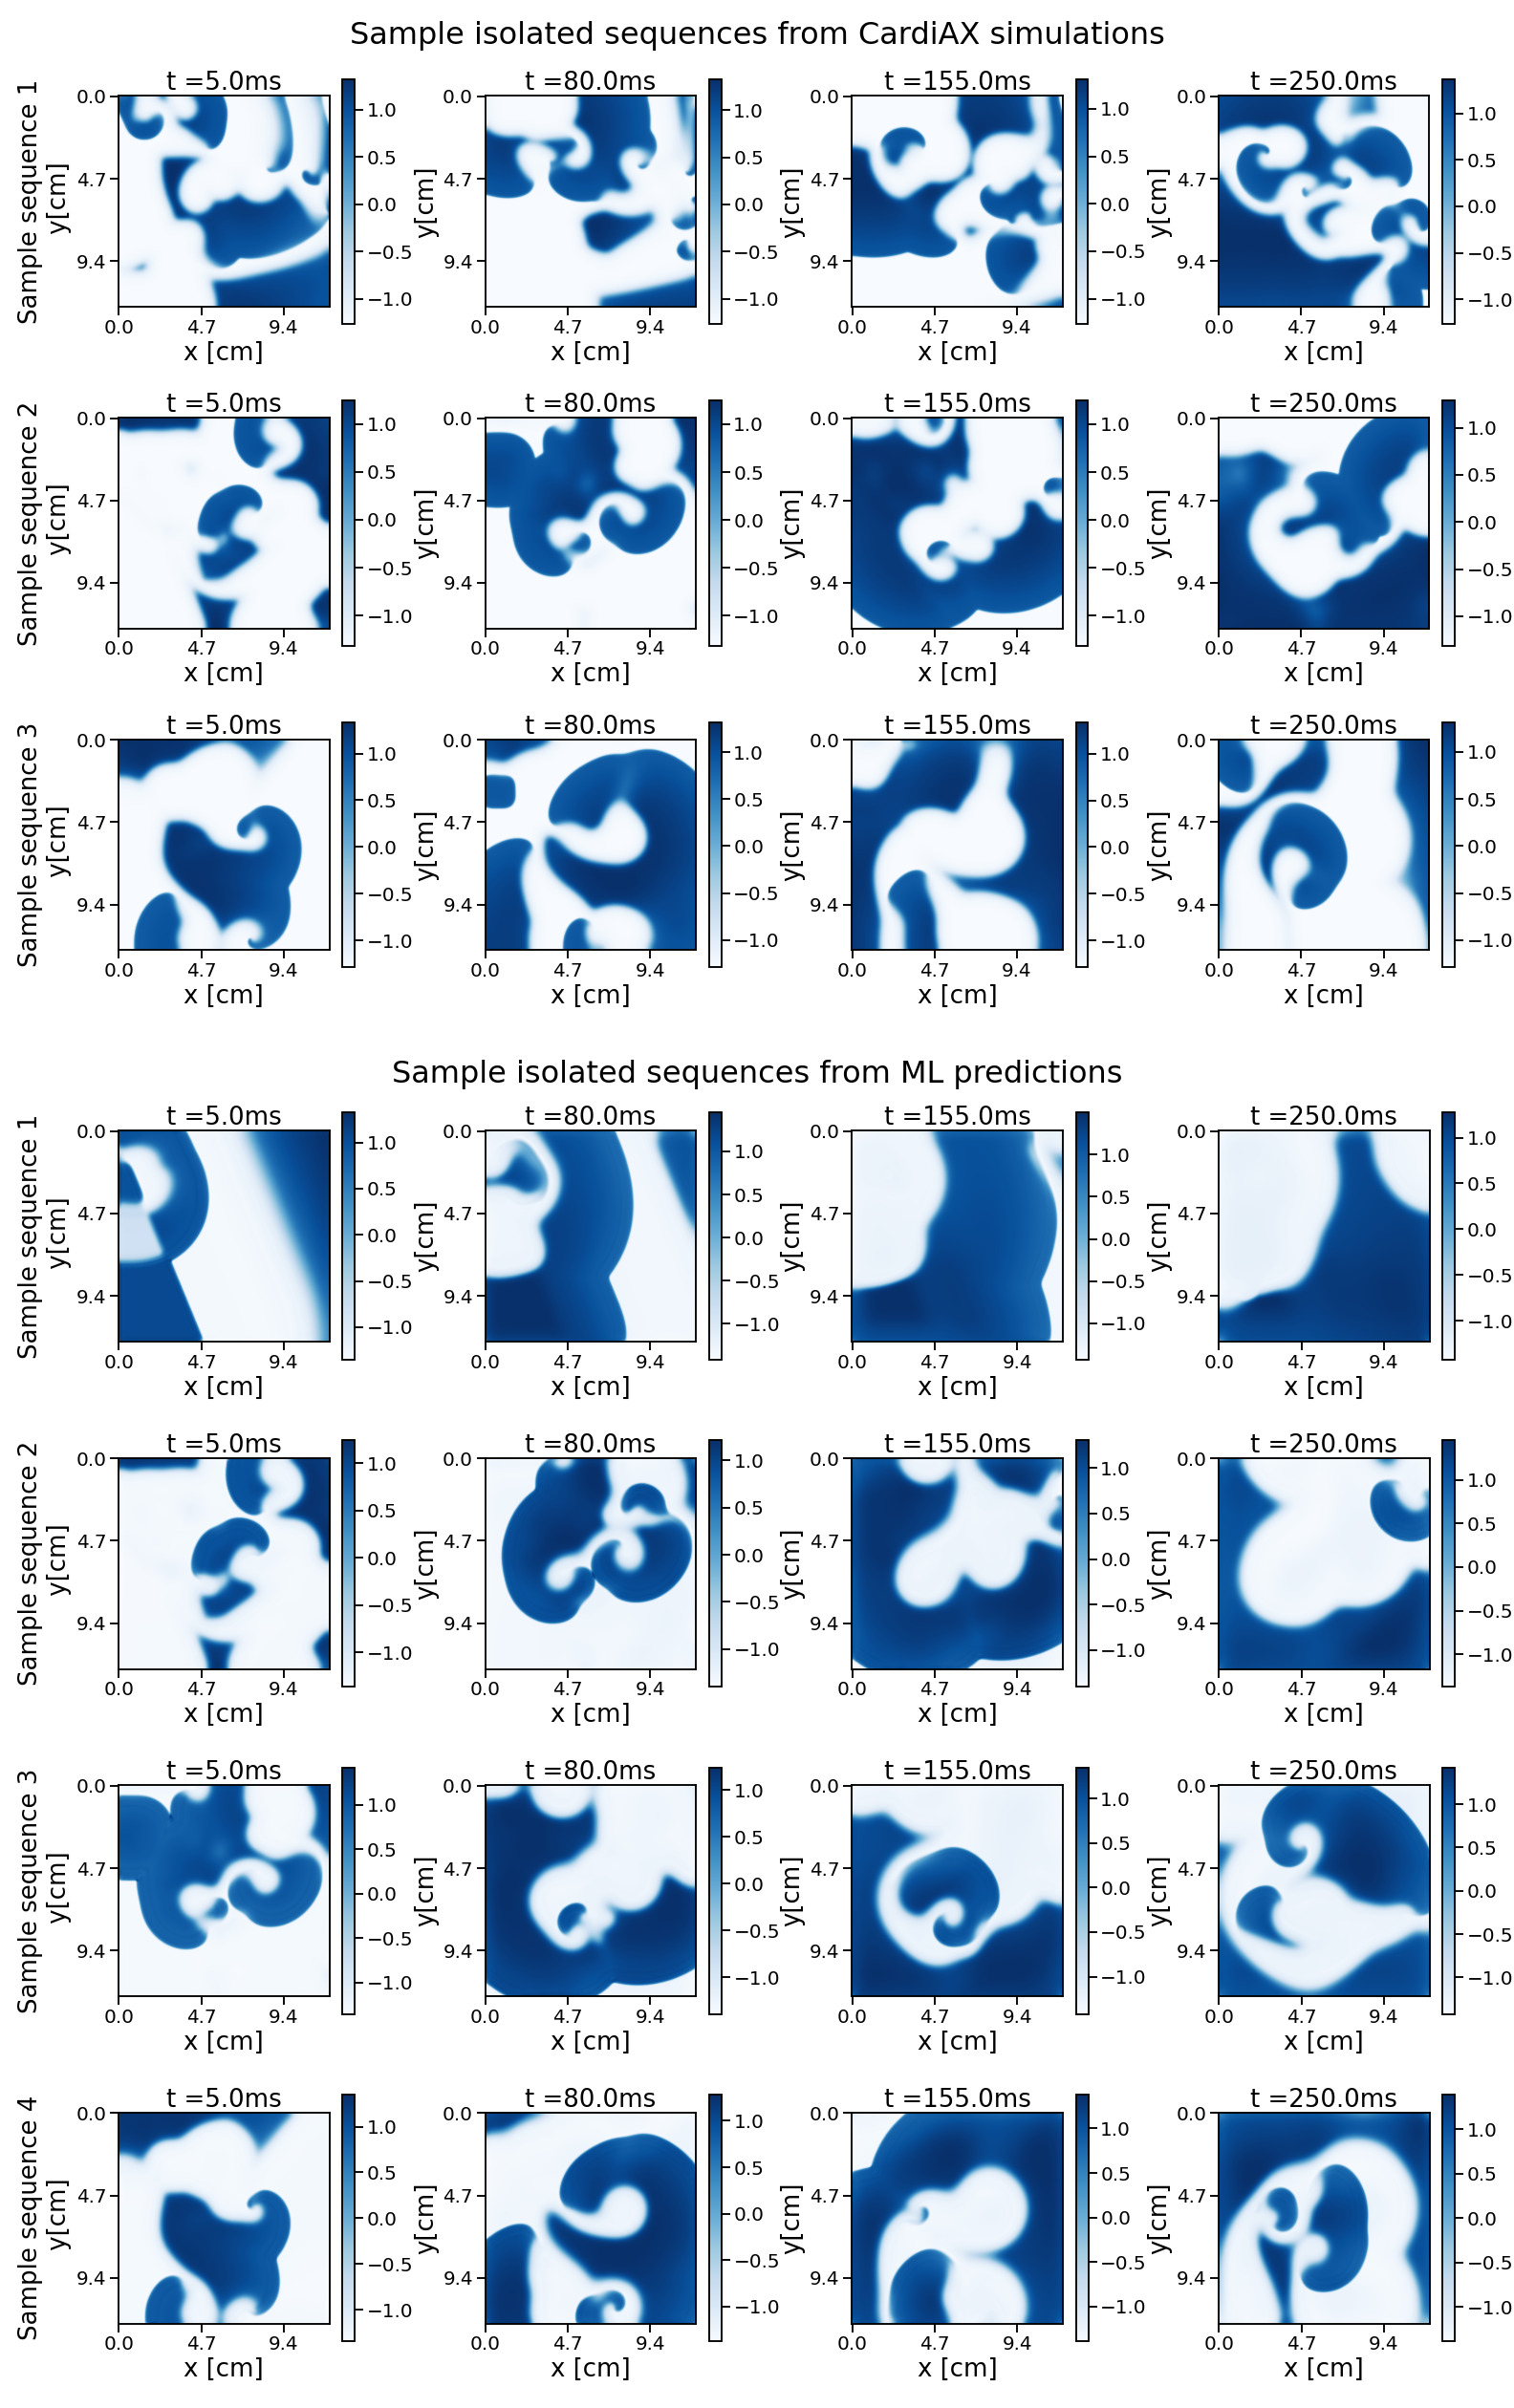
\includegraphics[width=.8\textwidth]{figures/old_figures/Figure-6.jpg}
\caption{Examples of sequences whose spectral signature is distinctive of \textit{CardiAX} simulations (top) and ML predictions (bottom). Note how some sequences appear in both sets but diverge over time (e.g. row two for the \textit{CardiAX} simulation corresponds to row two for the ML predictions).}
\label{fig:isolatedsequences}
\end{figure}

We then use the spectral moments as a potential signature to identify ``isolated'' sequences generated either by \textit{CardiAX} or by the trained neural network, as described in section~\ref{ch:spectral}. The rationale is that these distinctive simulations might represent dynamical regimes exhibited by the \textit{CardiAX} simulations that are not captured by the neural network, and vice-versa. Identifying these sequences would allow for further investigation into possible failure points of the neural network model.
Out of $321$ sequences in total for each condition, there are $78$ and $162$ isolated sequences for \textit{CardiAX} simulations and neural network predictions, respectively. Fig \ref{fig:isolatedsequences} shows some representative samples from each. Notice how some sequences appear in both sets but diverge over time. For example, the \textit{CardiAX} simulation in the second row (top figure) shows additional wave fronts that do not appear in the corresponding neural network prediction (second row, bottom figure). Further engineering of the Gamma distributions used to weigh contributions from different frequency bands might help refine these results.

Overall, the proof-of-principle experiments described in this section show that our neural network architecture seems capable of modelling complex dynamics in the case of homogeneous diffusivity, albeit with sensitivity to small perturbations that cause accumulation of errors over time.



\subsection{Computational performance}
We measured the computational costs of solving the Fenton-Karma equations using the optimised neural network, and compared to \textit{CardiAX}.
The neural network and \textit{CardiAX} share the same software infrastructure \cite[]{jax2018github}, which removes many unknowns from the comparison.
Tests are run on a single GPU environment using a \textit{NVIDIA GeForce GTX 1070 Ti}.
We predict the state of the system, varying the size of the tissue and registering the values every 5ms, up to 100ms.
A single test is composed by five serial runs of the same code, for both the finite difference solution and the neural network one.
After an initial system warm-up, we choose the solution with the lowest computational time among the five runs, as reported in the official python documentation \cite[]{10.5555/1593511} at: \url{https://docs.python.org/3/library/timeit.html#timeit.Timer.repeat}. Choosing the lowest value equals selecting a lower bound for how fast the machine can perform on the given code.
No results are cached between different runs.
We study how the computation scales with the size of the grid, starting from a grid size of $2^4$ and increasing it exponentially until the calculations reach the GPU memory limit.

\begin{minipage}[htp!]{\textwidth}
\begin{minipage}[tp]{0.49\textwidth}
\centering
\vspace{0.2cm}
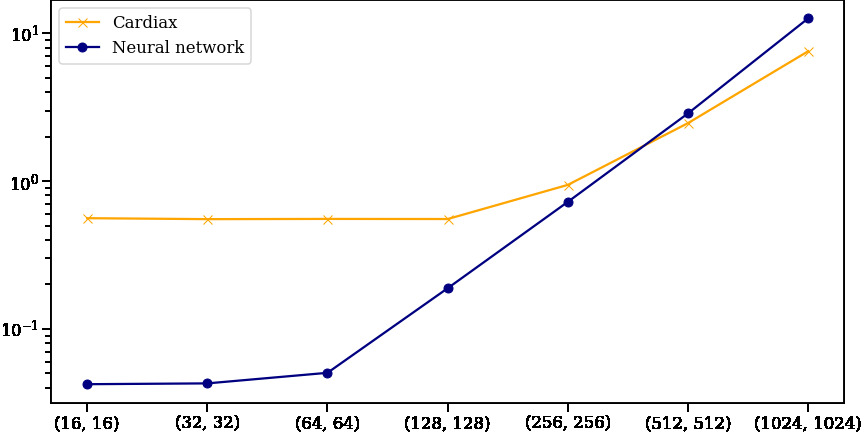
\includegraphics[width=\textwidth]{figures/old_figures/Figure-11.jpg}
\captionof{figure}{
    Computational cost in seconds for calculating the solution of the PDE after 100ms. The image shows the evolution of the costs by varying the number of points in the grid. 
}
\label{fig:performance}
\end{minipage}
\hfill
\begin{minipage}[tp]{0.49\textwidth}
\centering
\tiny
\begin{tabular}{l r r}                    
    \hline
    \textbf{\# Grid points} & \textbf{CardiAX} & \textbf{Neural Network} \\
    \hline
    $(16, 16)$ & $0.557$s & $\textbf{0.042}$s \\ [2pt]
    $(32, 32)$ & $0.552$s & $\textbf{0.043}$s \\ [2pt]
    $(64, 64)$ & $0.556$s & $\textbf{0.050}$s \\ [2pt]
    $(128, 128)$ & $0.548$s & $\textbf{0.188}$s \\ [2pt]
    $(256, 256)$ & $0.931$s & $\textbf{0.726}$s \\ [2pt]
    $(512, 512)$ & $\textbf{2.471}$s & $2.881$s \\ [2pt]
    $(1024, 1024)$ & $\textbf{7.588}$s & $12.663$s \\
    \hline
\end{tabular}
\captionof{table}{
    Computational cost in seconds for calculating the solution of the PDE after 100ms. The table shows the values of the plot on the left. Best results are in bold; lower is better.
}
\label{tab:performance}
\end{minipage}
\end{minipage}
\vspace{0.5cm}

Results show that \textit{CardiAX} saturates the GPU memory later than the neural network, marking shape (128, 128) compared to (32, 32).
The neural network is very efficient in a low dimensional regime, where finite difference performs an order of magnitude worse.
Times are comparable at 256 points, and  diverge afterwards, with the neural network performing slightly worse.


% -------
\section{Supplementary Tables and Figures}

% For more information on Supplementary Material and for details on the different file types accepted, please see \href{http://home.frontiersin.org/about/author-guidelines#SupplementaryMaterial}{the Supplementary Material section} of the Author Guidelines.

% Figures, tables, and images will be published under a Creative Commons CC-BY licence and permission must be obtained for use of copyrighted material from other sources (including re-published/adapted/modified/partial figures and images from the internet). It is the responsibility of the authors to acquire the licenses, to follow any citation instructions requested by third-party rights holders, and cover any supplementary charges.

% %% Figures, tables, and images will be published under a Creative Commons CC-BY licence and permission must be obtained for use of copyrighted material from other sources (including re-published/adapted/modified/partial figures and images from the internet). It is the responsibility of the authors to acquire the licenses, to follow any citation instructions requested by third-party rights holders, and cover any supplementary charges.

% \subsection{Figures}

% %%% There is no need for adding the file termination, as long as you indicate where the file is saved. In the examples below the files (logo1.eps and logos.eps) are in the Frontiers LaTeX folder
% %%% If using *.tif files convert them to .jpg or .png
% %%%  NB logo1.eps is required in the path in order to correctly compile front page header %%%

% \begin{figure}[htbp]
% \begin{center}
% 
\includegraphics[width=9cm]{logo1}% This is a *.eps file
% \end{center}
% \caption{ Enter the caption for your figure here.  Repeat as  necessary for each of your figures}\label{fig:1}
% \end{figure}


% \begin{figure}[htbp]
% \begin{center}
% \includegraphics[width=10cm]{logos}
% \end{center}
% \caption{This is a figure with sub figures, \textbf{(A)} is one logo, \textbf{(B)} is a different logo.}\label{fig:2}
% \end{figure}

% %%% If you are submitting a figure with subfigures please combine these into one image file with part labels integrated.
% %%% If you don't add the figures in the LaTeX files, please upload them when submitting the article.
% %%% Frontiers will add the figures at the end of the provisional pdf automatically
% %%% The use of LaTeX coding to draw Diagrams/Figures/Structures should be avoided. They should be external callouts including graphics.


%\bibliographystyle{frontiersinSCNS_ENG_HUMS} %  for Science, Engineering and Humanities and Social Sciences articles, for Humanities and Social Sciences articles please include page numbers in the in-text citations
\bibliographystyle{frontiersinHLTH&FPHY} % for Health and Physics articles
\bibliography{references}


\end{document}
